% !Mode:: "TeX:UTF-8"
%%  本模板推荐以下方式编译:
%%     1. PDFLaTeX[推荐]
%%     2. xelatex [含中文推荐]
%%  注意:
%%  1. 文件默认的编码为 UTF-8 对于windows,请选用支持UTF-8编码的编辑器。
%%   2. 若是模板有什么问题,请及时与我们取得联系,Email:latexstudio@qq.com。
%%   3. 可以到  https://ask.latexstudio.net 提问
%%   4. 请安装 最新版本的 TeXLive 地址:
%%   http://mirrors.ctan.org/systems/texlive/Images/texlive.iso

\documentclass{apmcmthesis}

\usepackage{url}
\usepackage{CJK}
\usepackage{appendix}
\usepackage{listings}%插入代码
\usepackage{xcolor} 
\usepackage{graphicx}%插入表格
\usepackage{booktabs} %绘制表格
\usepackage{caption} %标题
\usepackage{geometry}
\usepackage{array}
\usepackage{amsmath}
\usepackage{amssymb}
\usepackage{subfigure} %插入图片
\usepackage{longtable}
\usepackage{abstract}%摘要
\usepackage{setspace}
\usepackage{multirow}%表格
\usepackage{diagbox}
\usepackage{enumerate}%序号
\usepackage{float}%固定图片或表格的位置
\usepackage{gensymb}
\usepackage{microtype}
\def\oc{$^{\circ}$C\;}

%%%%%%%%%%%%填写相关信息%%%%%%%%%%%%%%%%%%%%%%%%%%
\tihao{C}                            %选题
\baominghao{2212335}                 %参赛编号
\begin{document}

\renewcommand{\abstractname}{abstract}
\pagestyle{frontmatterstyle}

\begin{abstract}

\verb|apmcmthesis| \LaTeX{} template is designed by \url{https://www.latexstudio.net} for \url{http://www.apmcm.org}. The template is designed to let everyone focus on the content writing of the paper, without spending too much effort on the customization and adjustment of the format.

Note that users need to have some experience with \LaTeX{}, at least some of the features of common macro packages, such as references, math formulas, image usage, list environment, etc. Templates have added commonly used macros. Package, no additional user added.

This template is located on   \url{https://github.com/latexstudio/APMCMThesis}. You can update files from the repository.


\keywords{Keywords1\quad  Keywords2\quad   Keywords3}

\end{abstract}



\newpage
%目录
\tableofcontents


\newpage
\pagestyle{mainmatterstyle}
\setcounter{page}{1}
\section{Introduction}
In order to indicate the origin of problems, the following background is worth mentioning.

Since this year, we have seen a large number of amazing temperature reports. 
There is no doubt that the earth is burning. 
Following the terrible high temperature in these areas from the end of June to the beginning of July, 
Italy set a European temperature record again, reaching an astonishing 48.8 ° C, 
and many countries declared a state of emergency.

Global warming is a phenomenon related to nature. 
It is precisely because of the continuous accumulation of the greenhouse effect that the energy absorbed and emitted by the Earth's atmospheric system is unbalanced. 
The continuous accumulation of the energy of the Earth's atmospheric system leads to temperature rise and global warming.

Before the industrial revolution, the carbon dioxide (CO2) in the atmosphere was about 280 parts per million. 
In March 2004, the atmospheric CO2 concentration reached 377.7ppm, the largest average increase in 10 years so far. 
According to the statistics of scientists from the National Oceanic and Atmospheric Administration (NOAA) and the Scripps Institution of Oceanography (SIO), 
the monthly average concentration of CO2 reached a peak of 421ppm in May 2022. 
An OECD report predicted that the CO2 concentration would reach 685ppm by 2050.

\section{Question restatement}

1) Do you agree with the global temperature statement? 
Data given in attachment and other data sets collected by the team analyze changes in global temperature.
Are you suggesting that the rise in global temperature in March 2022 has caused more growth than any decade ago.
Based on historical data, please develop two or more mathematical models to show the past and predict the future level of global temperature.
Use each model at 1(b) to estimate global temperature in 2050 and 2100.
Which model of 1(b) do you think is the right one, and why.

2) What are the causes that affect temperature change?
Use the results of question 1 and annex Data. 
Data from other data sets collected by csv and your team, developed a mathematical model to verify the relationship between global temperature, 
time and location (whatever), and explain the relationship between them or prove that there is no relationship between them.
Collect native data and check actions that have an impact on natural disasters (such as volcanic eruptions, forest fires and COVID-19). 
Does it affect global temperature? 
What do you think is the main reason that is affecting global temperature change?
Do you think there are steps that can stop or slow global warming?

3) Prepare a non-technical article (mostly on 1 page). Write a non-technical article (mostly on 1 page) 
to the APMCM Organization Committee to explain your team's findings and suggestions for the future.
The PDF solution with a total number of not more than 25 pages contains: 
a full table of one page; and complete solution catalogue; A non-technical article page.

\section{Terms, definitions and symbols}

\section{Models assumptions}

\section{Solution for question 1}
In whole question 1, we need to analyze global temperature changes using dataset in the attachment and other datasets we collect.

\subsection{(a)}
\subsubsection{Analysis of problem 1(a)}
In this question, we need to judge if the increase of global temperature in March 2022 resulted in a larger increase thean observed over any previous 10-year period. 
So we can plot the global temperature in 2022.
Firstly, consider if global temperature in March 2022 is a abnormal value. 
Then calculate the average temperature between 2011 to 2021 and its rising rate.
We let them be visual and analyze their trend and differences. 
Finally we conclude a agreement of the statement. 

\subsubsection{Solution of problem}
We download global temperature dataset from \url{https://berkeleyearth.org/data/}.
And we choose land only monthly average temperature to plot the figure. 
The picture about annual average temperature between 1760 to 2022 is the following.

\begin{figure}[htbp]
  \centering
  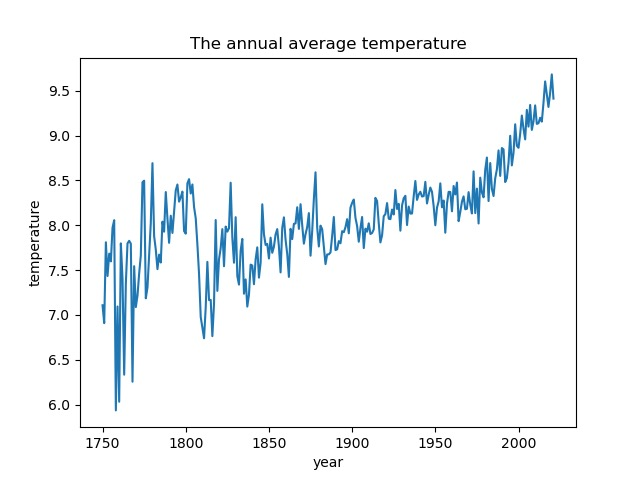
\includegraphics[scale=0.4]{annual avg tem.jpg}
  \caption*{picture 1}\label{fig1}
\end{figure}

Then we get the average temperature in March between 2011 to 2021 is the following. 

\begin{align*}
  [6.0780,5.9890, 6.2030, 6.3420 , 6.7220 ,7.4750 , 7.1340 , 6.6680 , 7.0950  ,7.0450 ,6.6840].
\end{align*}

\begin{figure}[htbp]
  \centering
  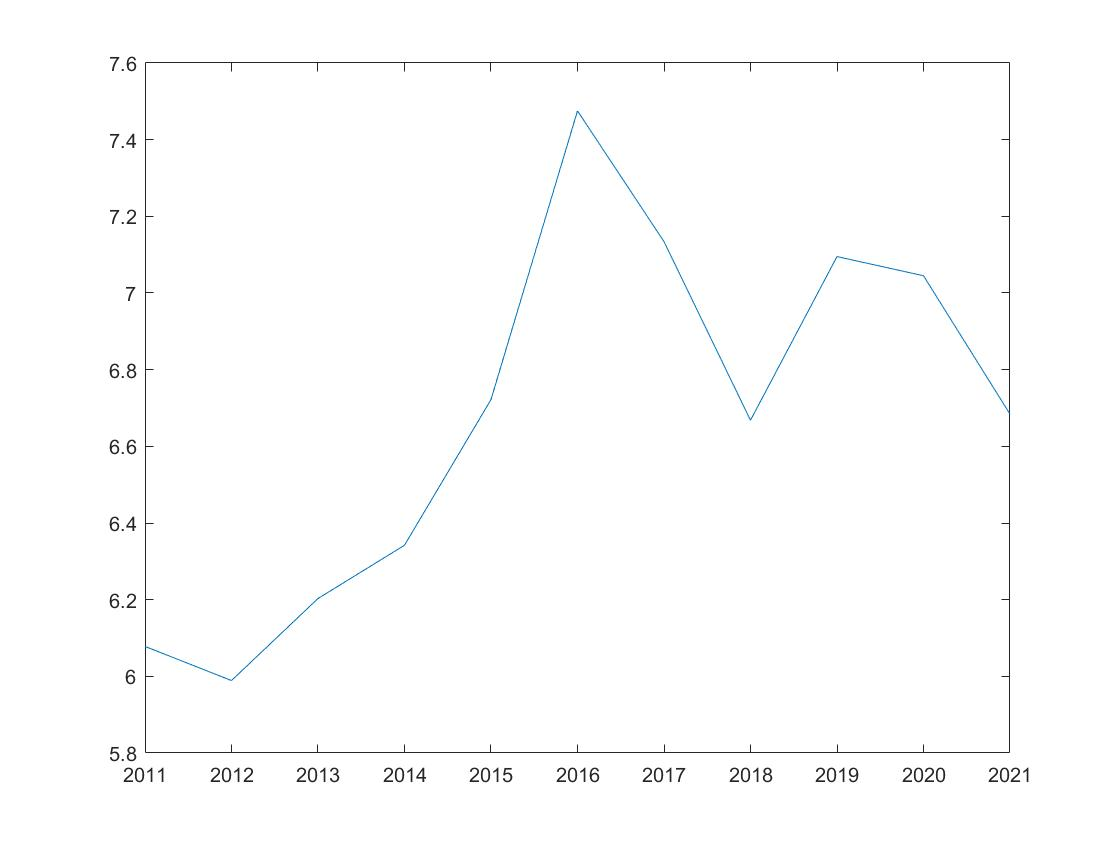
\includegraphics[scale=0.2]{past 10 avg.jpg}
  \caption*{picture 2}\label{fig2}
\end{figure}

The total increasing rate is 1.100\%, and increase 0.606\oc in value.
Increasing rate respectively is given by
\begin{align*}
  [ -0.0941,-0.0146,0.0357,0.0224,0.0599,0.1120, -0.0456,-0.0653, 0.0640,-0.0070,-0.0512].
\end{align*}
Past 10 years average temperature is 6.6759\oc. 

And the monthly average temperature between January 2022 to October 2022 except March we can calculate is 
\begin{align*}
  [3.989,  4.358, 6.812,9.665, 12.313, 14.742, 15.588, 15.07 ,13.151, 10.811].
\end{align*}
\begin{figure}[htbp]
  \centering
  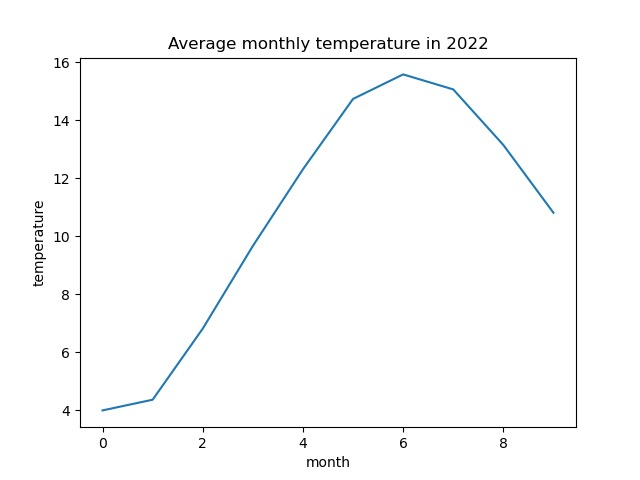
\includegraphics[scale=0.35]{Average monthly temperature in 2022.jpg}
  \caption*{picture 3}\label{fig3}
\end{figure}

Especially, the increasing rate between 2022 to 2021 is 0.0192.
This is much smaller than previous 10 years.


\subsection{(b)}
\subsubsection{Analysis of problem 1(b)}
Question (b) require us to build 2 or more mathematical models to describe the past and predict the future global temperature level.
We can pick a observation as example to analyze the data annually. 
That is we build models using yearly average temperature. 
We decide to use Autoregressive integrated moving average (ARIMA) model and Gray forecast model(GFM) to describe the global temperature.

\subsubsection{Model 1: SARIMA}

ARIMA model, differential integrated moving average autoregression model, also known as integrated moving average autoregression model, 
is one of the time series prediction and analysis methods.
In ARIMA (p, d, q), AR is `autoregressive', and p is the number of autoregressive terms; 
MA is the `moving average', q is the number of moving average terms, and d is the number of differences (orders) made to make it a stationary sequence.
This model is built to describe the relationship between current value and historical value using the historical time data of the variable itself to predict itself.
So it fit to the question in 1(b).

Firstly, we need to determine the order p which means the lagged order i.e how many previous variable related to the current value.
This leads an autoregressive model(AR):
\begin{align*}
  y_t = \mu + \sum^p_{i=1} \gamma_i y_{t-i} + \epsilon_t
\end{align*}
where $y_t$ is current value, $\mu$ is constant.

Then we consider more about the error along the time series. 
We get the moving average model(MA):
\begin{align*}
  y_t = \mu + \sum^q_{i=1} \theta_i \epsilon_{t_i} + \epsilon_t
\end{align*}
This can reduce the random fluctuation when estimating. 

Finally, we combine previous 2 models then obtain the model ARMA
\begin{align*}
  y_t = \mu + \sum^p_{i=1} \gamma_i y_{t-i}  + \sum^q_{i=1} \theta_i \epsilon_{t_i} + \epsilon_t
\end{align*}

But this model has some limitations.
The results that ARMA obtains might not be stationary, then some test will not be credible. 
So we can add a difference order d to let them be stationary. 

We load the dataset `land year std data'

Before we obtain the expression of ARIMA, we need to determine the value of p, q and d.
In general, we choose low value of d i.e low order for the model. 
So it is important to find a reasonable value of p, q.
We can check the Akaike information criterion(AIC) and Schwarz criterion(SC) 
given by respectively:
\begin{align*}
  AIC&=\ln(\frac{SSE}{T})+\frac{2K}{T},\;\;\;\;K=p+q+2.\\
  SC&=\ln(\frac{SSE}{T})+\frac{K\ln(T)}{T}.
\end{align*}
If AIC and SC are small enough, then the choices of p and q are preferred.
So we can use the force algorithm to find the best combination of p, q.

Moreover we need to check which model we should use to estimate the data.
We can check the autocorrelation function(ACF):
\begin{align*}
  ACF(k)=\rho_k = \frac{Cov(y_t,y_{t-k})}{Var(y_t)}.
\end{align*}
k is the lagged index.
We calculate the statistic ACF and plot a scatter so that we can really determine which model is the better one.

After we get the annual average temperature, we first perform a stationarity check on the data. The most intuitive way is to use the data to make a sequence diagram and then observe the trend of the image. At the same time, we calculate the first-order difference and the second-order difference of the data and make a graph to observe the trend.

\begin{figure}[htbp]
  \centering
  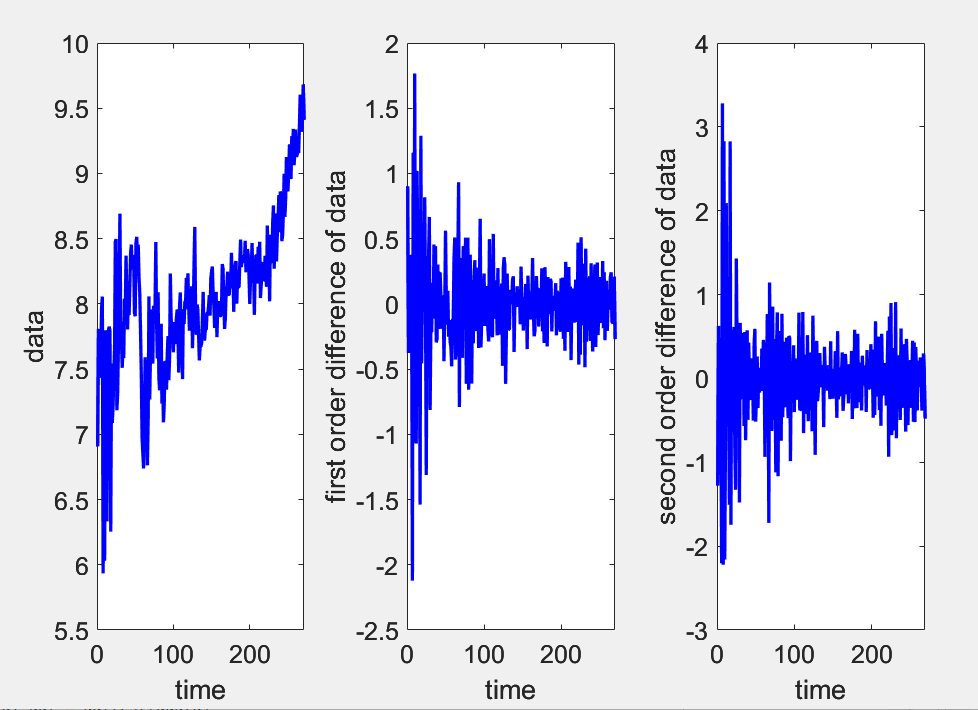
\includegraphics[scale=0.35]{Smoothness Analysis.png}
  \caption*{picture 4}\label{fig5}
\end{figure}

It is not obvious from the image to confirm the stationary relationship of the data, so we use the mathematical test method——ADF test and KPSS test.

In the ADF test, if the return value is 0, the data is not stationary, and if the return value is 1, the data is stationary. Then in KPSS test, if the return value is 0, the data is stationary, and if the return value is 1, the data is not stationary.

From the test result we can know the raw data is not stationary, so we need to calculate the first order difference of data, then we do the same test to the first order difference of data. We can get
\begin{figure}[htbp]
  \begin{minipage}[t]{0.45\linewidth}
    \centering
    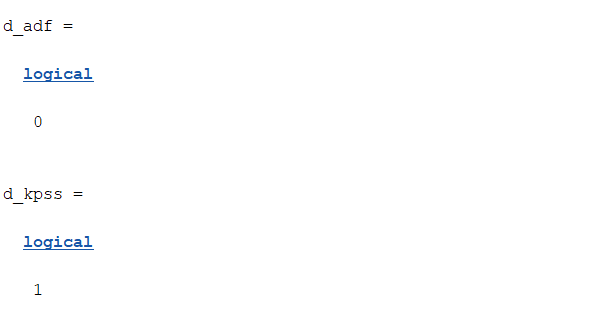
\includegraphics[scale=0.5]{order 1.png}
    \caption*{picture 5}
  \end{minipage}%
  \begin{minipage}[t]{0.45\linewidth}
    \centering
    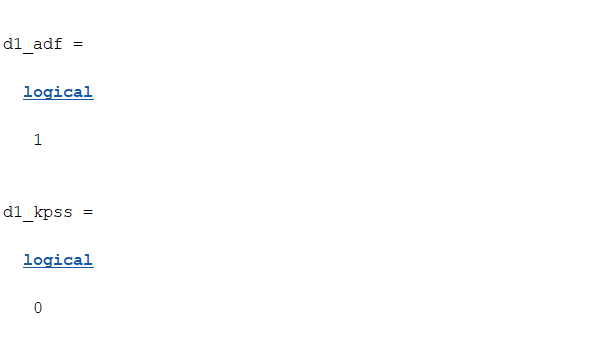
\includegraphics[scale=0.5]{order 2.png}
    \caption*{picture 6}
  \end{minipage}
\end{figure}

Therefore, the data after the first order difference can be used for time series modeling analysis. And then what we need to do is to confirm the parameters p q d. The first step is to examine the autocorrelation and partial autocorrelation plots of a stationary time series.

\begin{figure}[htbp]
  \centering
  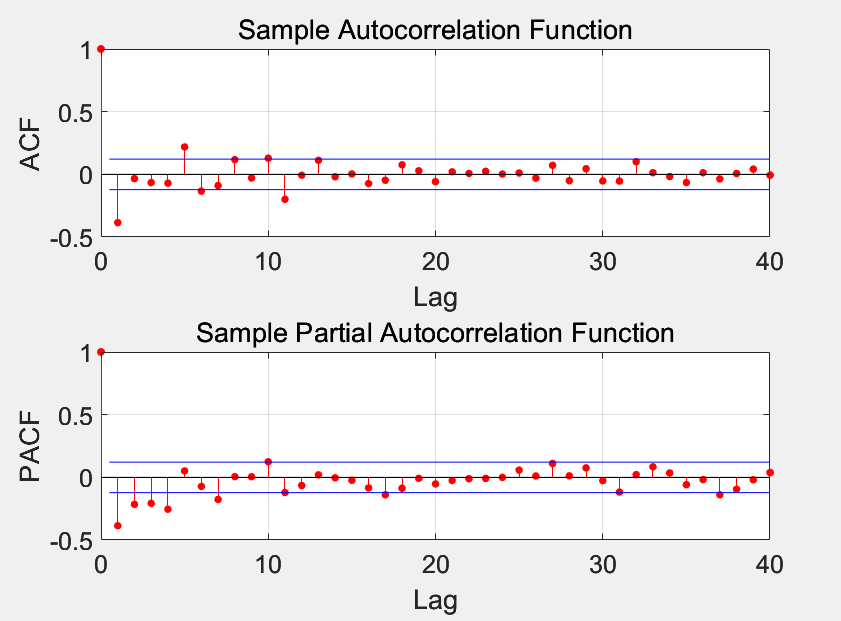
\includegraphics[scale=0.4]{ACF.png}
  \caption*{picture 7}\label{fig7}
\end{figure}

We can't get the values of p and q from the figure, so we adopt the AIC and BIC criteria to find the most suitable p and q values within a certain range. When we have confirmed the appropriate p q d value, we can build a model to predict the subsequent data. In the process of forecasting, we also set the upper and lower forecast limits under the 95% confidence interval.

First, let's predict the annual average temperature for the next 100 years.

\begin{figure}[htbp]
  \centering
  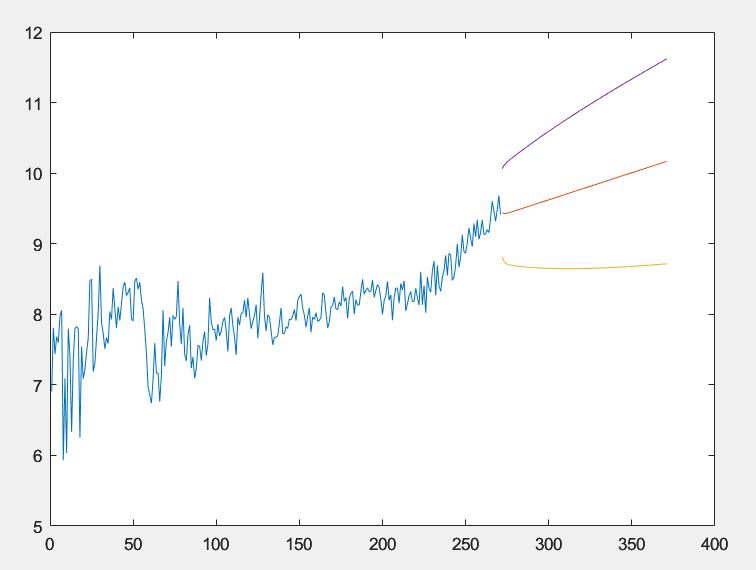
\includegraphics[scale=0.4]{ARIMA prediction 100.png}
  \caption*{picture 8}\label{fig8}
\end{figure}

\begin{figure}[htbp]
  \centering
  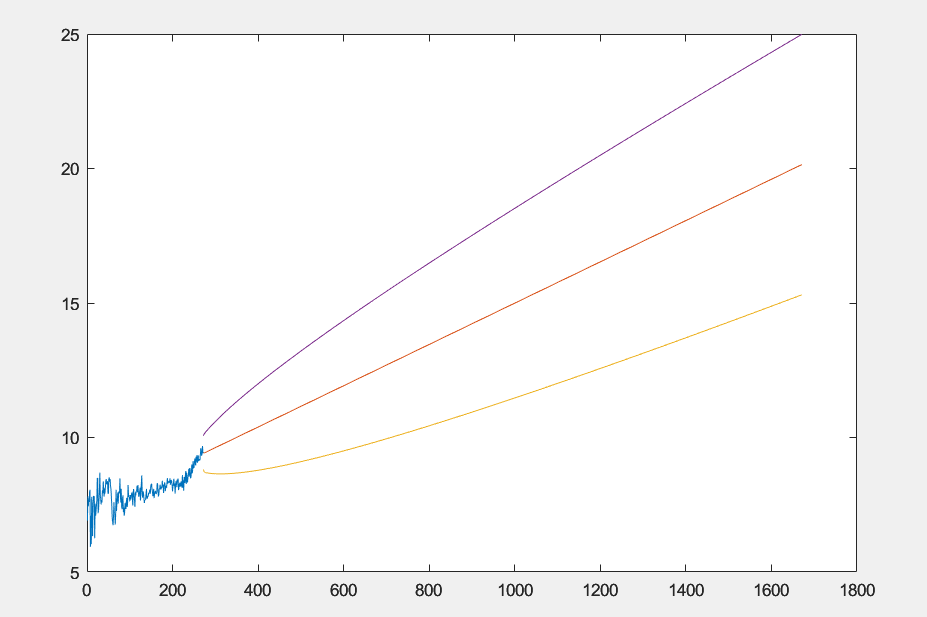
\includegraphics[scale=0.4]{ARIMA prediction 1400.png}
  \caption*{picture 9}\label{fig9}
\end{figure}


Then, we choose seasonal ARIMA to estimate the average global temperature.
This is because we obtain only stable prediction by ARIMA, while ARIMA cannot estimate seasonal data well.
So we do some extention to ARIMA, add a seasonal factor to ARIMA.
That is:
\begin{align*}
  y_t = \mu + \sum^p_{i=1} \gamma_i y_{t-i}  + \sum^p_{i=1} \Gamma_i y_{t-is} + \sum^q_{i=1} \theta_i \epsilon_{t_i} +  \sum^q_{i=1} \Theta_i \epsilon_{t-is} +\epsilon_t
\end{align*}

We can find that it is the multiple of ARIMA and seasonal expression $s(p,q,d)$.
This step does not be like obtaining ARIMA from ARMA, which just adds a differential operater d.
It mulitply seasonal factor s to ARIMA to get SARIMA.

\subsubsection{Model 2: }

\subsubsection{Description of global temperature in recent 100 years}
Using the models that we build in previous section, we draw the picture of past 50 years and future 50 years global temperature level.

 


\subsection{(c)}
According to the model in question 1(b), we can easily predict global temperatures in 2050 and 2100 respectively using different models. 
Moreover we need to find when the average temperature of observation points in ous prediction models will reach 20.00\oc.

\subsection{(d)}
We need to calculate important statistics to determine which model is better. 
We compare SE, MSE and RMSE and draw a figure as the following.


\section{Solution for question 2}
In question 2, we are required to build a global temperature model not only including the value of temperature 
but also more other reasons such as position, time, volcanic eruptions, forest fires and the COVID-19 etc.

\subsection{(a)}
\subsubsection{Analysis of problem 2(a)}
According to the data given in attachment 1, we analyze the correlation between  global temperature, time and location.
Draw a heat map, and use ridge regression in multiple linear regression to describe the relationship between variable above.
We decide to use Pearson correlation coefficient to describe the relationship between temperature, time and location.
This is because the values of them do affect each other, and the order of temperature is an important factor that judge the relastionship. 
Moreover, time temperature and location must satisfy some linear relationship, so we decide to use Pearson correlation coefficient to describe. 

And we want to analyze further to prove the correctness of the relationship. 
So we use Grey relation analysis(GRA) to make sure that they really have some relationship.

\subsubsection{Test of Pearson correlation coefficient}

\subsubsection{Test of Grey relation analysis}



\subsection{(b)}
\subsubsection{Data of natural disasters}
In this section, we should get data of the natural disasters, we find part of data(such as volcanic eruptions, forest fires) in \url{https://www.emdat.be/}, and part of data(COVID-19) in \url{https://covid19.who.int/data}.




\subsection{(c)}
\subsubsection{Data of more factor}
We find datasets of world energy, world population and Global forest resource. 
\url{https://www.bp.com/en/global/corporate/energy-economics/statistical-review-of-world-energy/downloads.html}
\url{https://population.un.org/wpp/Download/Standard/MostUsed/}
\url{https://fra-data.fao.org/WO/fra2020/dataDownload/} 

\subsubsection{}


\subsection{(d)}



\newpage
\section{Solution for question 3}



\section{Future Work}
\subsection{Another model}
\subsubsection{The limitations of queuing theory}




\subsubsection{}


\subsubsection{}



\subsubsection{}





%参考文献
\begin{thebibliography}{9}%宽度9
\bibitem{1} Author, Title, Place of Publication: Press, Year of publication.
\bibitem{2} author, paper name, magazine name, volume number: starting and ending
page number, year of publication.
\bibitem{3} author, resource title, web site, visit time (year, month, day).
\bibitem{bib:one} \LaTeX{}{资源和技巧学习} \url{https://www.latexstudio.net}
\bibitem{bib:two} \LaTeX{}{问题交流网站} \url{https://wenda.latexstudio.net}
\bibitem{bib:two} {模板库维护} \url{https://github.com/latexstudio/APMCMThesis}
\end{thebibliography}

\newpage
%附录

\section{Appendix}
\begin{lstlisting}[language=matlab,caption={The matlab Source code of Algorithm}]
kk=2;[mdd,ndd]=size(dd);
while ~isempty(V)
[tmpd,j]=min(W(i,V));tmpj=V(j);
for k=2:ndd
[tmp1,jj]=min(dd(1,k)+W(dd(2,k),V));
tmp2=V(jj);tt(k-1,:)=[tmp1,tmp2,jj];
end
tmp=[tmpd,tmpj,j;tt];[tmp3,tmp4]=min(tmp(:,1));
if tmp3==tmpd, ss(1:2,kk)=[i;tmp(tmp4,2)];
else,tmp5=find(ss(:,tmp4)~=0);tmp6=length(tmp5);
if dd(2,tmp4)==ss(tmp6,tmp4)
ss(1:tmp6+1,kk)=[ss(tmp5,tmp4);tmp(tmp4,2)];
else, ss(1:3,kk)=[i;dd(2,tmp4);tmp(tmp4,2)];
end;end
dd=[dd,[tmp3;tmp(tmp4,2)]];V(tmp(tmp4,3))=[];
[mdd,ndd]=size(dd);kk=kk+1;
end; S=ss; D=dd(1,:);
 \end{lstlisting}
\begin{lstlisting}[language=c,caption={The lingo source code}]
kk=2;
[mdd,ndd]=size(dd);
while ~isempty(V)
    [tmpd,j]=min(W(i,V));tmpj=V(j);
for k=2:ndd
    [tmp1,jj]=min(dd(1,k)+W(dd(2,k),V));
    tmp2=V(jj);tt(k-1,:)=[tmp1,tmp2,jj];
end
    tmp=[tmpd,tmpj,j;tt];[tmp3,tmp4]=min(tmp(:,1));
if tmp3==tmpd, ss(1:2,kk)=[i;tmp(tmp4,2)];
else,tmp5=find(ss(:,tmp4)~=0);tmp6=length(tmp5);
if dd(2,tmp4)==ss(tmp6,tmp4)
    ss(1:tmp6+1,kk)=[ss(tmp5,tmp4);tmp(tmp4,2)];
else, ss(1:3,kk)=[i;dd(2,tmp4);tmp(tmp4,2)];
end;
end
    dd=[dd,[tmp3;tmp(tmp4,2)]];V(tmp(tmp4,3))=[];
    [mdd,ndd]=size(dd);
    kk=kk+1;
end;
S=ss;
D=dd(1,:);
 \end{lstlisting}


\end{document} 